% Homecastr Investor Pitch Deck - V6
% Compile with: xelatex homecastr_pitch_v6.tex

\documentclass[aspectratio=169,12pt]{beamer}

% ─── Theme & Colors ──────────────────────────────────────────
\usetheme{default}
\usecolortheme{default}
\setbeamertemplate{navigation symbols}{}
\setbeamertemplate{footline}{%
  \ifnum\thepage>1\relax%
    \hbox to \paperwidth{%
      \kern1em\href{https://homecastr.com}{\includegraphics[height=0.35cm]{assets/homecastr-logo-horizontal.png}}%
      \hfill%
      {\usebeamercolor[fg]{page number in head/foot}\usebeamerfont{page number in head/foot}\insertframenumber}%
      \kern1em%
    }\vskip2pt%
  \fi%
}
\setbeamertemplate{frametitle}{
  \vspace{10pt}
  \begin{beamercolorbox}[wd=\paperwidth,center]{frametitle}
    \usebeamerfont{frametitle}\insertframetitle
    \par\vspace{4pt}
    {\color{hcGold}\hrule height 1.5pt width 4cm}
  \end{beamercolorbox}
}

% Homecastr brand palette — matched to website CSS
\definecolor{hcBg}{HTML}{F2EDE4}        % --background
\definecolor{hcText}{HTML}{3D3830}       % --foreground
\definecolor{hcGold}{HTML}{CA8A04}       % accent gold (CTAs, stats)
\definecolor{hcGoldLight}{HTML}{E8D5A0}
\definecolor{hcMuted}{HTML}{7E7B74}      % --muted-foreground
\definecolor{hcCard}{HTML}{E8E2D8}       % --muted / card bg
\definecolor{hcPrimary}{HTML}{6B6356}    % --primary (taupe)
\definecolor{hcRed}{HTML}{B91C1C}
\definecolor{hcGreen}{HTML}{15803D}

\setbeamercolor{background canvas}{bg=hcBg}
\setbeamercolor{normal text}{fg=hcText}
\setbeamercolor{frametitle}{fg=hcText}
\setbeamercolor{title}{fg=hcText}
\setbeamercolor{subtitle}{fg=hcMuted}
\setbeamercolor{itemize item}{fg=hcGold}
\setbeamercolor{itemize subitem}{fg=hcGold}
\setbeamertemplate{itemize item}{\raisebox{1pt}{\tikz{\node[regular polygon, regular polygon sides=6, fill=hcGold, inner sep=0pt, minimum size=3.5pt] {};}}}
\setbeamertemplate{itemize subitem}{\raisebox{1pt}{\tikz{\node[regular polygon, regular polygon sides=6, fill=hcGold, inner sep=0pt, minimum size=2.5pt] {};}}}


\setbeamerfont{title}{size=\Huge,series=\bfseries}
\setbeamerfont{frametitle}{size=\Large,series=\bfseries}
\setbeamerfont{subtitle}{size=\large}

% Packages
\usepackage{fontspec}
\setmainfont{Segoe UI}
\setsansfont{Segoe UI}
\usepackage{tikz}
\usetikzlibrary{calc,positioning,arrows.meta,shapes.geometric}
\usepackage{graphicx}
\usepackage{booktabs}
\usepackage{hyperref}
\hypersetup{colorlinks=true, urlcolor=hcGold, linkcolor=hcGold}

% ─── Macros ──────────────────────────────────────────────────
\newcommand{\goldtext}[1]{{\color{hcGold}#1}}
\newcommand{\mutedtext}[1]{{\color{hcMuted}#1}}
\newcommand{\statbox}[2]{%
  \begin{minipage}[t]{\linewidth}
    \centering
    {\LARGE\bfseries\color{hcGold}#1}\\[2pt]
    {\small\color{hcMuted}#2}
  \end{minipage}%
}

% Logo image macro (cropped to content)
\newcommand{\buildingicon}{%

\includegraphics[height=1.4cm]{assets/homecastr-icon.png}%
}

% Bottom-of-slide tagline — pushes to bottom of remaining frame space
\newcommand{\slidetagline}[1]{%
  \vspace*{0pt plus 1fill}%
  \begin{center}{\small\color{hcMuted}#1}\end{center}%
}

% Big stat macro for single-stat visual slides
\newcommand{\bigstat}[2]{%
  {\fontsize{64}{72}\selectfont\bfseries\color{hcGold}#1}\\[8pt]
  {\Large\color{hcText}#2}%
}

% ══════════════════════════════════════════════════════════════
\begin{document}

% ─── SLIDE 1: Title ──────────────────────────────────────────
\usebackgroundtemplate{\includegraphics[width=\paperwidth,height=\paperheight]{assets/title_bg.png}}
\begin{frame}[plain]
\vfill
\begin{center}
\includegraphics[height=2cm]{assets/homecastr-logo-horizontal.png}\\[16pt]
{\Large\color{hcText} The foundation model for property forecasting}\\[24pt]
\mutedtext{\small \href{https://homecastr.com}{\textcolor{hcGold}{\textbf{homecastr.com}}}}
\end{center}
\vfill
\end{frame}

% ─── Default background for remaining slides ─────────────────
% Use \color+\rule fill — works in one pass, no TikZ overlay needed
\usebackgroundtemplate{\color{hcBg}\rule{\paperwidth}{\paperheight}}


% ─── SLIDE 2: Live Today ─────────────────────────────────────
\begin{frame}{Live today}
\vspace{8pt}

\begin{columns}[c]
\begin{column}{0.63\textwidth}
\centering
\href{https://homecastr.com}{\includegraphics[width=\linewidth,height=5cm,keepaspectratio=true]{assets/dashboard_screenshot.png}}
\end{column}
\begin{column}{0.34\textwidth}
\centering
\statbox{15\%$^{*}$}{median error at 4yr}\\[14pt]
\statbox{4yr}{forecast horizon}\\[14pt]
\statbox{1M+}{properties forecasted}\\[14pt]
{\tiny\color{hcMuted}\centering $^{*}$50\% of properties fall below this error.}
\end{column}
\end{columns}

\slidetagline{\href{https://homecastr.com}{\textcolor{hcGold}{homecastr.com}} \textbar{} Houston metro. Live. Free.}
\end{frame}


% ─── SLIDE 3: The Gap ────────────────────────────────────────
\begin{frame}{Everyone knows what a home is worth today}
\vspace{4pt}

\begin{center}
{\large\color{hcText} Nobody can affordably show you where it's \goldtext{going}.}
\end{center}

\vspace{12pt}

\begin{columns}[c]
\begin{column}{0.44\textwidth}
\begin{center}
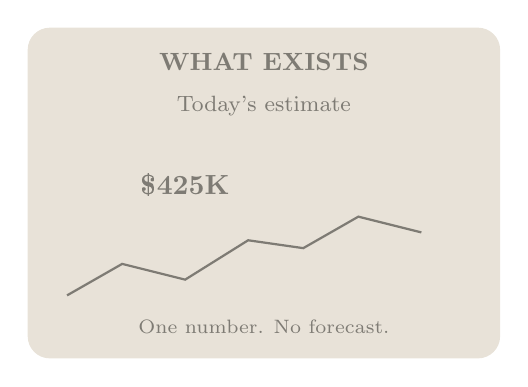
\begin{tikzpicture}
  % "Today" box — static point estimate
  \fill[hcCard, rounded corners=8pt] (0,0) rectangle (6.0,4.2);
  \node[anchor=north, font=\small\bfseries, text=hcMuted] at (3.0,4.0) {WHAT EXISTS};
  \draw[hcMuted, thick] (0.5,0.8) -- (1.2,1.2) -- (2.0,1.0) -- (2.8,1.5) -- (3.5,1.4) -- (4.2,1.8) -- (5.0,1.6);
  \node[font=\footnotesize, text=hcMuted, align=center] at (3.0,3.2) {Today's estimate};
  \node[font=\normalsize\bfseries, text=hcMuted] at (2.0,2.2) {\$425K};
  \node[font=\scriptsize, text=hcMuted] at (3.0,0.4) {One number. No forecast.};
\end{tikzpicture}
\end{center}
\end{column}
\begin{column}{0.08\textwidth}
\begin{center}
{\fontsize{28}{32}\selectfont\color{hcGold}\textbf{→}}
\end{center}
\end{column}
\begin{column}{0.44\textwidth}
\begin{center}
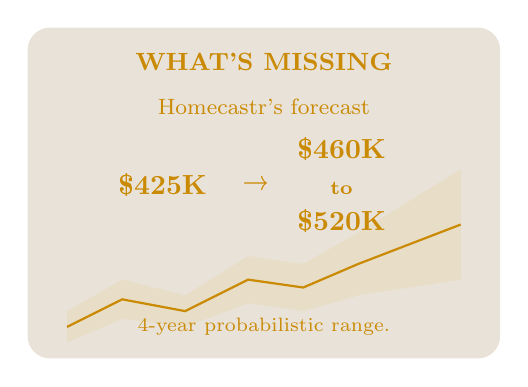
\begin{tikzpicture}
  % "Tomorrow" box — forecast bands
  \fill[hcCard, rounded corners=8pt] (0,0) rectangle (6.0,4.2);
  \node[anchor=north, font=\small\bfseries, text=hcGold] at (3.0,4.0) {WHAT'S MISSING};
  % Forecast band fill
  \fill[hcGoldLight, opacity=0.3] (0.5,0.6) -- (1.2,1.0) -- (2.0,0.8) -- (2.8,1.3) -- (3.5,1.2) -- (4.2,1.6) -- (5.5,2.4)
    -- (5.5,1.0) -- (4.2,0.8) -- (3.5,0.6) -- (2.8,0.7) -- (2.0,0.4) -- (1.2,0.5) -- (0.5,0.2) -- cycle;
  % Median forecast line
  \draw[hcGold, thick] (0.5,0.4) -- (1.2,0.75) -- (2.0,0.6) -- (2.8,1.0) -- (3.5,0.9) -- (4.2,1.2) -- (5.5,1.7);
  \node[font=\footnotesize, text=hcGold, align=center] at (3.0,3.2) {Homecastr's forecast};
  \node[font=\normalsize\bfseries, text=hcGold, anchor=east] at (2.4,2.2) {\$425K};
  \node[font=\normalsize, text=hcGold] at (2.9,2.2) {→};
  \node[font=\normalsize\bfseries, text=hcGold, align=center, anchor=west] at (3.3,2.2) {\$460K\\[1pt]{\scriptsize to}\\[1pt]\$520K};
  \node[font=\scriptsize, text=hcGold] at (3.0,0.4) {4-year probabilistic range.};
\end{tikzpicture}
\end{center}
\end{column}
\end{columns}

\end{frame}


% ─── SLIDE 3: How It Works (expanded) ───────────────────────
\begin{frame}{How it works}
\vspace{8pt}

% ── Pipeline row ──
\begin{center}
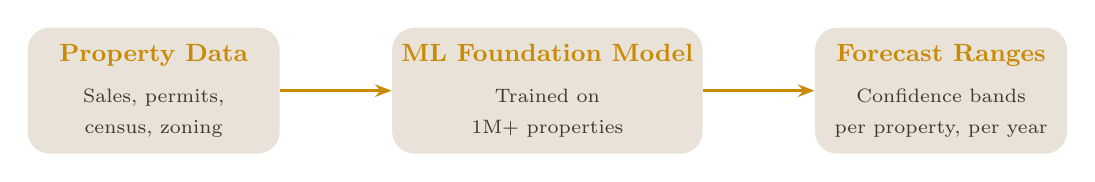
\begin{tikzpicture}[
  block/.style={rounded corners=8pt, fill=hcCard, text=hcText,
    minimum width=3.2cm, minimum height=1.6cm, align=center, font=\small},
  arr/.style={-{Stealth[length=6pt]}, very thick, color=hcGold}
]
  \node[block] (data) at (0,0) {
    \goldtext{\textbf{Property Data}}\\[4pt]
    {\scriptsize Sales, permits,}\\
    {\scriptsize census, zoning}
  };
  \node[block] (model) at (5,0) {
    \goldtext{\textbf{ML Foundation Model}}\\[4pt]
    {\scriptsize Trained on}\\
    {\scriptsize 1M+ properties}
  };
  \node[block] (output) at (10,0) {
    \goldtext{\textbf{Forecast Ranges}}\\[4pt]
    {\scriptsize Confidence bands}\\
    {\scriptsize per property, per year}
  };
  \draw[arr] (data) -- (model);
  \draw[arr] (model) -- (output);
\end{tikzpicture}
\end{center}

\end{frame}


% ─── SLIDE 5: Why Now ────────────────────────────────────────
\begin{frame}{Why now}
\vspace{12pt}

\begin{columns}[c]
\begin{column}{0.50\textwidth}
\begin{center}
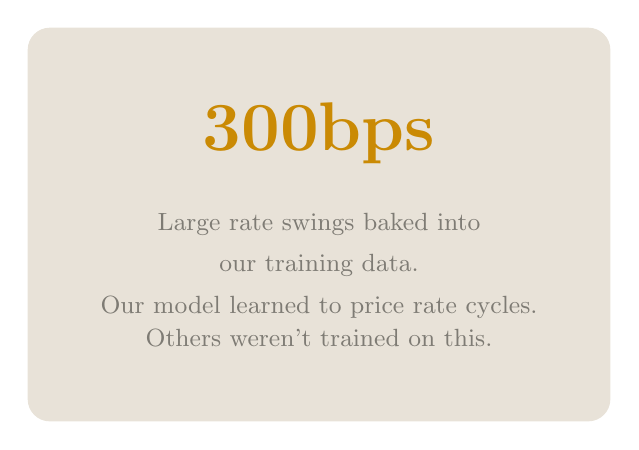
\begin{tikzpicture}
  \fill[hcCard, rounded corners=8pt] (0,0) rectangle (7.4,5.0);
  \node at (3.7,2.5) {%
    \begin{minipage}[c][4.2cm][c]{6.8cm}\centering
      {\fontsize{30}{34}\selectfont\bfseries\color{hcGold} 300bps}\par
      \vspace{14pt}
      {\small\setlength{\baselineskip}{15pt}\color{hcMuted}
        Large rate swings baked into\\our training data.\\Our model learned to price rate cycles.\\Others weren't trained on this.}
    \end{minipage}%
  };
\end{tikzpicture}
\end{center}
\end{column}
\begin{column}{0.50\textwidth}
\begin{center}
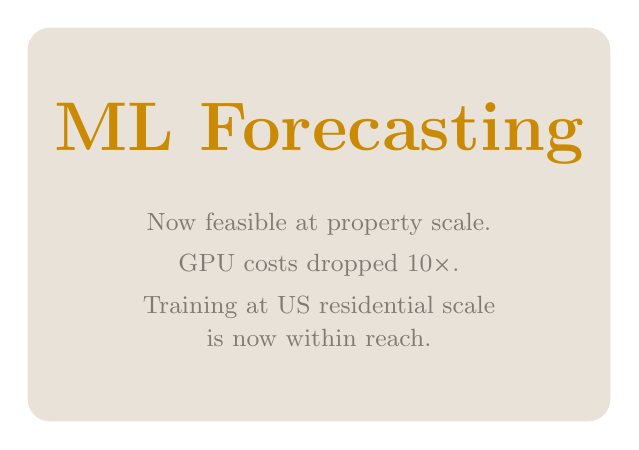
\begin{tikzpicture}
  \fill[hcCard, rounded corners=8pt] (0,0) rectangle (7.4,5.0);
  \node at (3.7,2.5) {%
    \begin{minipage}[c][4.2cm][c]{6.8cm}\centering
      {\fontsize{30}{34}\selectfont\bfseries\color{hcGold} ML Forecasting}\par
      \vspace{14pt}
      {\small\setlength{\baselineskip}{15pt}\color{hcMuted}
        Now feasible at property scale.\\GPU costs dropped 10{\texttimes}.\\Training at US residential scale\\is now within reach.}
    \end{minipage}%
  };
\end{tikzpicture}
\end{center}
\end{column}
\end{columns}


\end{frame}




% ─── SLIDE 6: Market ─────────────────────────────────────────
\begin{frame}{Market}
\vspace{12pt}

\begin{center}
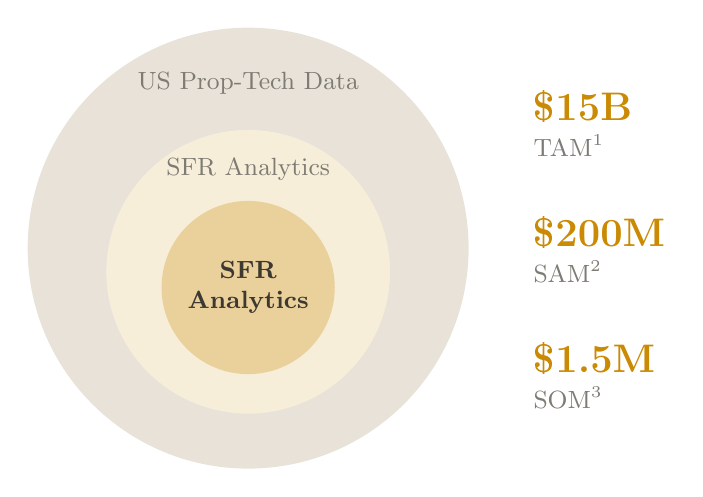
\begin{tikzpicture}
  % TAM
  \fill[hcCard] (0,0) circle (2.8cm);
  \node[text=hcMuted] at (0, 2.1) {\small US Prop-Tech Data};

  % SAM
  \fill[hcBg] (0,-0.3) circle (1.8cm);
  \fill[hcGoldLight!40] (0,-0.3) circle (1.8cm);
  \node[text=hcMuted] at (0, 1.0) {\small SFR Analytics};

  % SOM
  \fill[hcGold!40] (0,-0.5) circle (1.1cm);
  \node[text=hcText, font=\small\bfseries, align=center] at (0, -0.5) {SFR\\Analytics};

  % Labels
  \node[text=hcGold, font=\Large\bfseries, anchor=west] at (3.5, 1.8) {\$15B};
  \node[text=hcMuted, font=\small, align=left, anchor=west] at (3.5, 1.3) {TAM\textsuperscript{1}};

  \node[text=hcGold, font=\Large\bfseries, anchor=west] at (3.5, 0.2) {\$200M};
  \node[text=hcMuted, font=\small, anchor=west] at (3.5, -0.3) {SAM\textsuperscript{2}};

  \node[text=hcGold, font=\Large\bfseries, anchor=west] at (3.5, -1.4) {\$1.5M};
  \node[text=hcMuted, font=\small, anchor=west] at (3.5, -1.9) {SOM\textsuperscript{3}};
\end{tikzpicture}
\end{center}

\vspace{2pt}
\begin{center}
\mutedtext{\tiny\parbox{0.9\textwidth}{\setlength{\baselineskip}{7pt}%
\textsuperscript{1}\href{https://www.precedenceresearch.com/proptech-market}{US PropTech data market} (Precedence Research, 2025).\par
\textsuperscript{2}Est. SFR analytics segment: \href{https://www.corelogic.com}{CoreLogic} SFR div., \href{https://www.housecanary.com}{HouseCanary} (\$18M+), \href{https://www.attomdata.com}{ATTOM} (\$28M+), \href{https://www.propstream.com}{PropStream} (\$25M+).\par
\textsuperscript{3}{\raise.17ex\hbox{$\scriptstyle\sim$}}12K operators {\texttimes} \$99/mo {\texttimes} 10\% penetration, 10 metros. Annual revenue.}}
\end{center}
\end{frame}


% ─── SLIDE 7: Positioning (2x2 Quadrant) ────────────────────
\begin{frame}{Positioning}
\vspace{8pt}

\begin{center}
\begin{tikzpicture}[scale=0.9]
  % Axes
  \draw[hcMuted, thick, -{Stealth[length=5pt]}] (-4.5,0) -- (4.8,0);
  \draw[hcMuted, thick, -{Stealth[length=5pt]}] (0,-3.2) -- (0,3.8);

  % Axis labels
  \node[font=\footnotesize, text=hcMuted, anchor=north] at (-3.0,-0.15) {Backward-Looking};
  \node[font=\footnotesize, text=hcGold, anchor=north] at (3.8,-0.15) {Predictive};
  \node[font=\footnotesize, text=hcMuted, anchor=east, rotate=90] at (-0.2,-1.5) {Sales-Led};
  \node[font=\footnotesize, text=hcGold, anchor=east, rotate=90] at (-0.2,3.5) {Product-Led};

  % Quadrant shading — golden quadrant (top-right)
  \fill[hcGoldLight, opacity=0.15] (0.1,0.1) rectangle (4.5,3.5);

  % CoreLogic: data infrastructure, moderately predictive, deeply sales-led
  \node[inner sep=1pt] at (1.5,-2.2)
    {\includegraphics[width=1.8cm,height=0.45cm,keepaspectratio]{assets/logo_corelogic.png}};

  % HouseCanary
  \node[inner sep=1pt] at (2.8,-1.8)
    {\includegraphics[width=1.8cm,height=0.45cm,keepaspectratio]{assets/logo_housecanary.png}};

  % PropStream: launched AI/predictive features late 2024 (foreclosure factor, wholesale value)
  \node[inner sep=1pt] at (-3.2,1.5)
    {
\includegraphics[width=1.8cm,height=0.45cm,keepaspectratio]{assets/logo_propstream.png}};

  % Zillow: mostly current-state Zestimate, very product-led
  \node[inner sep=1pt] at (-2.5,2.8)
    {\includegraphics[width=1.8cm,height=0.45cm,keepaspectratio]{assets/logo_zillow_v2.png}};

  % Reventure: now has 12-month ZIP-level forecasts (30K+ ZIPs), self-serve product
  % Shifted right to avoid covering the 'Product-Led' y-axis label near x=0
  \node[inner sep=2pt, fill=hcCard, rounded corners=2pt] at (1.2,2.5)
    {
\includegraphics[width=1.8cm,height=0.45cm,keepaspectratio]{assets/logo_reventure.png}};

  % Homecastr — golden quadrant hero (slightly larger bounding box)
  \node[anchor=south west] at (3.6,2.8) {\includegraphics[width=2.2cm,height=0.55cm,keepaspectratio]{assets/homecastr-logo-horizontal.png}};

\end{tikzpicture}
\end{center}


\end{frame}


% ─── SLIDE 8: Business Model ────────────────────────
\begin{frame}{Business model}
\vspace{12pt}

\begin{columns}[c]
\begin{column}{0.48\textwidth}
\begin{center}
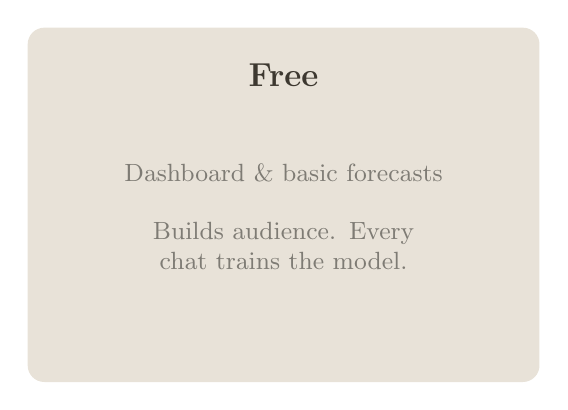
\begin{tikzpicture}
  \fill[hcCard, rounded corners=6pt] (0,0) rectangle (6.5,4.5);
  \node[font=\large\bfseries, text=hcText] at (3.25,3.9) {Free};
  \node[font=\small, text=hcMuted, align=center, text width=5.5cm] at (3.25,2.1) {Dashboard \& basic forecasts\\[10pt]Builds audience. Every chat trains the model.};
\end{tikzpicture}
\end{center}
\end{column}
\begin{column}{0.04\textwidth}
\begin{center}
{\color{hcGold}\textbf{$\rightarrow$}}
\end{center}
\end{column}
\begin{column}{0.48\textwidth}
\begin{center}
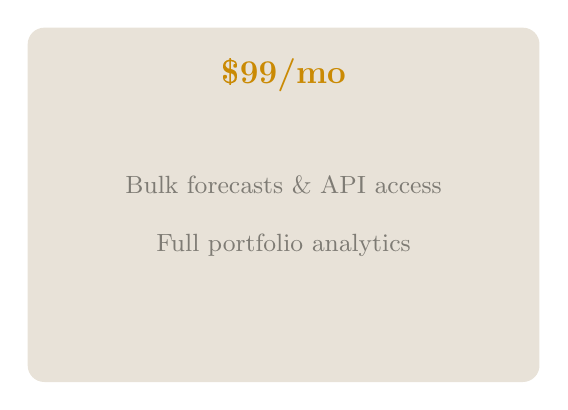
\begin{tikzpicture}
  \fill[hcCard, rounded corners=6pt] (0,0) rectangle (6.5,4.5);
  \node[font=\large\bfseries, text=hcGold] at (3.25,3.9) {\$99/mo};
  \node[font=\small, text=hcMuted, align=center, text width=5.5cm] at (3.25,2.1) {Bulk forecasts \& API access\\[10pt]Full portfolio analytics};
\end{tikzpicture}
\end{center}
\end{column}
\end{columns}

\end{frame}


% (Where We Are moved to slide 2 — see above)


% ─── SLIDE 10: Flywheel ─────────────────────────────────────
\begin{frame}{Flywheel}
\vspace{8pt}

\begin{center}
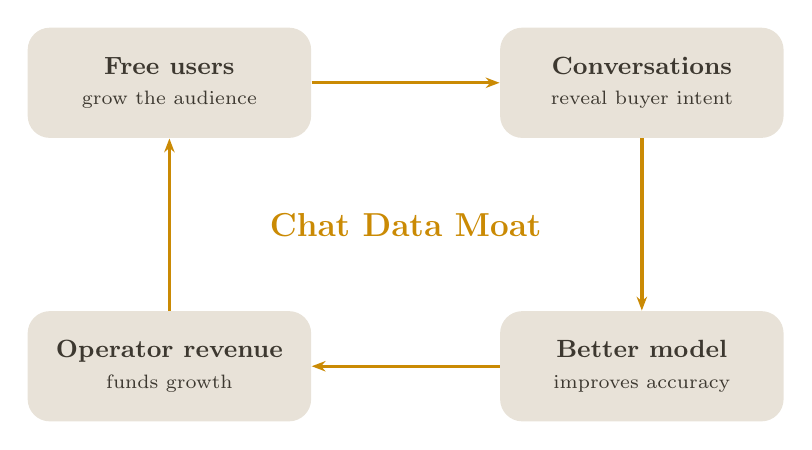
\begin{tikzpicture}[
  block/.style={rounded corners=8pt, fill=hcCard, text=hcText,
    minimum width=3.6cm, minimum height=1.4cm, align=center, font=\small},
  arr/.style={-{Stealth[length=5pt]}, very thick, color=hcGold}
]
  \node[block] (consumers) at (-3.0,1.8) {\textbf{Free users}\\{\scriptsize grow the audience}};
  \node[block] (signal) at (3.0,1.8) {\textbf{Conversations}\\{\scriptsize reveal buyer intent}};
  \node[block] (model) at (3.0,-1.8) {\textbf{Better model}\\{\scriptsize improves accuracy}};
  \node[block] (value) at (-3.0,-1.8) {\textbf{Operator revenue}\\{\scriptsize funds growth}};

  \draw[arr] (consumers) -- (signal);
  \draw[arr] (signal) -- (model);
  \draw[arr] (model) -- (value);
  \draw[arr] (value) -- (consumers);

  % Center label
  \node[font=\large\bfseries, text=hcGold] at (0,0) {Chat Data Moat};
\end{tikzpicture}
\end{center}

\end{frame}


% ─── SLIDE 11: Go-to-Market ─────────────────────────────────
\begin{frame}{Go-to-market}
\vspace{16pt}

\begin{columns}[T, totalwidth=\textwidth]
\begin{column}{0.33\textwidth}
\begin{center}
{\goldtext{\textbf{Direct outreach}}}\\[8pt]
{\small\color{hcMuted} Direct calls to SFR operators. Referrals close pilots.}
\end{center}
\end{column}
\begin{column}{0.01\textwidth}
\centering{\color{hcCard!60}\vrule height 4cm}
\end{column}
\begin{column}{0.31\textwidth}
\begin{center}
{\goldtext{\textbf{Broker sharing}}}\\[8pt]
{\small\color{hcMuted} Agents share Homecastr's forecasts with clients, creating organic word-of-mouth.}
\end{center}
\end{column}
\begin{column}{0.01\textwidth}
\centering{\color{hcCard!60}\vrule height 4cm}
\end{column}
\begin{column}{0.33\textwidth}
\begin{center}
{\goldtext{\textbf{Operator upsell}}}\\[8pt]
{\small\color{hcMuted} Try free. Upgrade to \$99/mo when you need bulk forecasts or API access.}
\end{center}
\end{column}
\end{columns}

\end{frame}


% ─── SLIDE 12: Team ──────────────────────────────────────────
\begin{frame}{Team}
\vspace{8pt}

\begin{columns}[c]

% Left: headshot + name
\begin{column}{0.38\textwidth}
\begin{center}
\begin{tikzpicture}
  \node[circle, inner sep=0pt, minimum size=2.8cm, path picture={
    \node at (path picture bounding box.center) {\includegraphics[width=2.8cm]{assets/dhl.png}};
  }] {};
\end{tikzpicture}\\[8pt]
{\Large\bfseries\color{hcGold} Daniel Hardesty Lewis}\\[4pt]
{\large Founder \& CEO}\\[4pt]
\mutedtext{\small \href{https://linkedin.com/in/dhardestylewis}{linkedin.com/in/dhardestylewis}}
\end{center}
\end{column}

% Right: credential rows
\begin{column}{0.58\textwidth}
\begin{tabular}{@{}rl@{}}
  \includegraphics[height=0.85cm]{assets/logo_summit.png} &
  \begin{tabular}[c]{@{}l@{}}
    \textbf{Summit Geospatial}\\
    \mutedtext{\scriptsize Founder: highest-quality terrain data, Texas}
  \end{tabular}\\[14pt]
  \colorbox{hcCard}{\includegraphics[height=0.7cm]{assets/logo_tacc.png}} &
  \begin{tabular}[c]{@{}l@{}}
    \textbf{Data Scientist, TACC}\\
    \mutedtext{\scriptsize Lead on \$40M FEMA resiliency project}
  \end{tabular}\\[14pt]
  \includegraphics[height=0.7cm]{assets/logo_egu.png} &
  \begin{tabular}[c]{@{}l@{}}
    \textbf{Scientific ML}\\
    \mutedtext{\scriptsize Bagnold Medal contributor, EGU}
  \end{tabular}\\
\end{tabular}
\end{column}

\end{columns}
\end{frame}


% ─── SLIDE 13: The Ask ──────────────────────────────────────
\begin{frame}[c]
\vspace{4pt}

\begin{center}
{\fontsize{36}{42}\selectfont\bfseries\color{hcGold} Raising \$1.75M}\\[8pt]
{\large Pre-Seed}
\end{center}

\vspace{10pt}

\begin{columns}[T]
\begin{column}{0.49\textwidth}
\textbf{Use of Funds}\\[6pt]
\begin{itemize}\setlength{\itemsep}{6pt}
  \item \textbf{ML Engineer}\\\mutedtext{Expand model to 10 metros}
  \item \textbf{GTM / Sales}\\\mutedtext{Land first 300 paying operators}
  \item \textbf{Data \& Compute}\\\mutedtext{Data licenses + GPU compute}
\end{itemize}
\end{column}
\begin{column}{0.48\textwidth}
\textbf{18-Month Milestones}\\[6pt]
\begin{itemize}\setlength{\itemsep}{6pt}
  \item \goldtext{\textbf{10 metros}}\\\mutedtext{20M+ properties}
  \item \goldtext{\textbf{\$30K MRR}}\\\mutedtext{from operator tier}
  \item \goldtext{\textbf{1 institutional pilot}}\\\mutedtext{or LOI}
\end{itemize}

\end{column}
\end{columns}

\vspace{4pt}
\begin{center}
\href{https://homecastr.com}{\goldtext{homecastr.com}} \quad|\quad \href{mailto:daniel@homecastr.com}{\mutedtext{daniel@homecastr.com}}
\end{center}
\end{frame}


% ─── SLIDE 14: Closing Title (Mirror of Slide 1) ────────────
\usebackgroundtemplate{\includegraphics[width=\paperwidth,height=\paperheight]{assets/title_bg.png}}
\begin{frame}[plain]
\vfill
\begin{center}
\includegraphics[height=2cm]{assets/homecastr-logo-horizontal.png}\\[16pt]
{\Large\color{hcText} The foundation model for property forecasting}\\[24pt]
\mutedtext{\small \href{https://homecastr.com}{\textcolor{hcGold}{\textbf{homecastr.com}}}}
\end{center}
\vfill
\end{frame}

\end{document}
